%  SingleXBs
%  Created by Dave Williams on 2009-06-25.
%  This is the source document for a paper about multi-spring
%  (and thus multi-dimensional) cross-bridges. These multi-spring 
%  cross-bridges are able to model forces that occur orthogonal 
%  to the direction of contraction in muscle. Additionally, the 
%  various properties of these cross-bridges change as muscle swells 
%  or contracts. 
% 
% header (fold)
\documentclass[10pt]{article}

% PLoS Formatting
% -------------------------------------------
% PLoS Suggested Packages
\usepackage{amsmath}
\usepackage{amssymb}
\usepackage{graphicx}

% PLoS Required Packages
\usepackage{cite}
\usepackage{color}

% Text layout
\topmargin 0.0cm
\oddsidemargin 0.5cm
\evensidemargin 0.5cm
\textwidth 16cm 
\textheight 21cm

% Bold the 'Figure #' in the caption and separate it with a period
% Captions will be left justified
\usepackage[labelfont=bf,labelsep=period,justification=raggedright]{caption}

% Use the PLoS provided bibtex style
\bibliographystyle{plos}

% Remove brackets from numbering in List of References
\makeatletter
\renewcommand{\@biblabel}[1]{\quad#1.}
\makeatother

% End of PLoS Formatting
% -------------------------------------------


% Necessary packages
\usepackage{fancyhdr}
\usepackage[utf8]{inputenc}

% Bibliography formatting
% Alternative to natbib, which is not PLoS simpatico
\newcommand{\citep}[1]{\cite{#1}} %natbib compatibility
\newcommand{\citet}[1]{\cite{#1}}
%\usepackage[round,numbers,sort&compress]{natbib} 
%\bibliographystyle{biophysj} % Requires biophysj.bst in doc dir
%\renewcommand{\bibnumfmt}[1]{#1.} % Numbering as 1. not [1]


% Packages that we may want to turn on and off
%% Set margins to 1in
%\usepackage[margin=1in]{geometry}
%% Use Times as the font, lord knows why 
%\renewcommand{\rmdefault}{ptm}
%% Use endfloat to put figures and tables at the end of the document
%\usepackage[nomarkers,tablesfirst,notablist,noheads]{endfloat}
%% Allow setting of H in float placement
%\usepackage{float}
%% Double or 1.5 space text
%\usepackage{setspace}
%\doublespacing
%% Multi-part figures
%\usepackage{subfigure}
%% Package for including code in the document
%\usepackage{listings}
%% Package for pdf output with embedded links 
%\usepackage[colorlinks=false, bookmarks=true, pdftex]{hyperref}

% Commands to make things easier and set lengths
\newcommand{\de}{$^\circ$} % \ensuremath kills latex2png
\addtolength{\parskip}{\baselineskip}
\setlength{\parindent}{0in}

% PLoS likes the title in the main doc
%\title{Lattice spacing and multi-dimensional forces in the cross-bridge} 

% Set short title as running header
\pagestyle{myheadings}
\markright{Cross-bridge forces depend on lattice spacing}

% PLoS likes author information in the main doc
%\author{C.~David Williams\thanks{
%            Corresponding Author. 
%            Email: cdave@uw.edu }\\ 
%        Department of Physiology and Biophysics, \\
%        University of Washington, Seattle, Washington
%        \and Michael Regnier \\
%        Department of Bioengineering, \\
%        University of Washington, Seattle, Washington
%        \and Thomas L.\ Daniel\\
%        Department of Biology, \\
%        University of Washington, Seattle, Washington
%        }

\date{} % Leave date blank

% header (end)

\begin{document}

% \maketitle{} % PLoS likes to do this manually
\begin{flushleft}
{\Large
\textbf{Axial and Radial Forces of Cross-bridges Depend on Lattice Spacing}
}
% Insert Author names, affiliations and corresponding author email.
\\
C.\ David Williams$^{1,\ast}$, 
Michael Regnier$^{1,2}$, 
Thomas L.\ Daniel$^{2,3}$
\\
\bf{1} Department of Physiology and Biophysics, University of Washington, Seattle, Washington, United States of America
\\
\bf{2} Department of Bioengineering, University of Washington, Seattle, Washington, United States of America
\\
\bf{3} Department of Biology, University of Washington, Seattle, Washington, United States of America
\\
$\ast$ E-mail: cdave@uw.edu
\end{flushleft}

\section*{Abstract} % (fold)
Nearly all mechanochemical models of the cross-bridge treat myosin as a simple linear spring arranged parallel to the contractile filaments.
These single-spring models cannot account for the radial force that muscle generates (orthogonal to the direction of contraction) or the effects of changes in filament lattice spacing. 
We describe a more complex myosin cross-bridge model that uses multiple springs to replicate myosin's force-generating power stroke and account for the effects of lattice spacing and radial force. 
The four springs which comprise this model (the 4sXB) correspond to the mechanically relevant portions of myosin's structure.
As occurs \emph{in vivo}, the 4sXB's state-transition kinetics and force production dynamics vary with lattice spacing.

Additionally, we describe a simpler two spring cross-bridge (2sXB) model which produces results similar to those of the 4sXB model.
Unlike the 4sXB model, the 2sXB model requires no iterative techniques, making it more computationally efficient.
The rate at which both multi-spring cross-bridges bind and generate force decreases as lattice spacing grows. 
The axial force generated by each cross-bridge as it undergoes a power stroke increases as lattice spacing grows.
The radial force that a cross-bridge produces as it undergoes a power stroke varies from expansive to compressive as lattice spacing increases.
Importantly, these results mirror those for intact, contracting muscle force production.

\emph{Keywords:} cross-bridge model; cross-bridge kinetics; lattice spacing; radial force; muscle model; myosin 
% section abstract (end)


\section*{Author Summary} % (fold)
The molecular motor myosin drives the contraction of muscle, but doesn't just produce force in the axis of shortening.
Models of muscle contraction have primarily treated myosin as a simple spring oriented parallel to its direction of movement. 
This assumption does not allow prediction of the relationship between the forces produced and the spacing between contractile filaments or of radial forces, perpendicular to the axis of shortening, which are observed during muscle contraction. 
We develop an alternative model, still computationally efficient enough to be used in simulations of the sarcomere, that incorporates both linear and torsional (angle dependent, like those found in a watch) springs. 
Our model captures much of the spacing dependent kinetics and forces that are missing from single-spring models of the cross-bridge.
% section author_summary (end)


\section*{Introduction} %(fold)

Radial forces are the same order of magnitude as axial forces in contracting muscles \citep{Maughan1981, Cecchi1990, Millman1998}. 
These forces, along with axial force in the direction of muscle contraction, depend on myofilament lattice spacing \citep{Bagni1994, Fuchs2005}. 
At the same time, structural information about myosin cross-bridges suggests that they generate force by applying torque to a lever arm \citep{Rayment1993, Uyeda1996, Huxley2000}.
This lever arm generates the strain accompanying the power stroke via a change in the rest angle at which the lever is attached to S1 region \citep{Huxley2000, Houdusse2001}. 
This change in angle occurs at the converter region, a flexible area in myosin S1 which acts as a torsional spring. 
These phenomena may be related: the radial forces a cross-bridge creates are results of the lever arm geometry (as suggested by Schoenberg \citep{Schoenberg1980b}). 

Existing theoretical and computational models of cross-bridge force generation at the level of the half-sarcomere assume that force is generated by a simple linear spring oriented parallel to the long axis of the myofilaments (Fig~\ref{fig_xb_types}A). 
This assumption has persisted from the earliest fundamental models of muscle contraction to more elaborate and spatially explicit models \citep{Huxley1957, Daniel1998, Chase2004, Tanner2007, Campbell2009}.  
These single-spring models yielded insight into the processes that regulate production of force in the direction of contraction.
However, these prior models of muscle contraction have paid less attention to radial forces and the effects of changes in filament lattice spacing. 
As a result, geometries of the single spring cross-bridge models have changed little while kinetic schemes governing transitions between conformational states have increased in complexity \citep{Huxley1957, Pate1989, Daniel1998, Smith2008a}. 
To analyze the radial forces that occur during muscle contraction, a different cross-bridge geometry is needed: a geometry that produces both forces aligned with and forces orthogonal to the direction of contraction. 
A lever arm of several springs can: (1) simulate the deformations a cross-bridge undergoes as it generates force through the power stroke, (2) provide a geometry which is practical for use in cross-bridge models, and (3) account for both axial and radial forces \citep{Houdusse2001}.  

Here we detail two models of cross-bridges that use multiple springs to replicate the lever arm mechanism and capture its biologically relevant effects (Fig~\ref{fig_xb_types}B-C).  
Both models are affected by changes in lattice spacing as well as axial offset from binding sites along the thin filament, and both account for the radial component of force produced during the power stroke.  
The first model (referred to as the 4sXB model) simulates the cross-bridge as a system of four linearly elastic springs arranged in a geometry based upon the structure of the S1 and S2 regions of myosin II (Fig~\ref{fig_xb_types}C).  
Our second model (referred to as the 2sXB model) consists of two linearly elastic springs and provides greater computational efficiency than the 4sXB model while replicating many of the more complex model's behaviors (Fig~\ref{fig_xb_types}B). 
The structure of the 2sXB model owes a debt to Schoenberg (1980) (\citep{Schoenberg1980a} and \citep{Schoenberg1980b}) which contain a proposal and analysis of a two spring cross-bridge where the S2 arm is represented as a linear spring and the S2-S1 junction is represented as a torsional spring. 
Both the 4sXB model and the 2sXB model use a three-state model of cross-bridge cycling kinetics, consisting of an unbound state, a low-force pre-power stroke state, and a force-producing post-power stroke state. 
The kinetics of transition from one state to another in our models are similar to those used previously but are generalized for use in two dimensions; our kinetics calculate transition probabilities using the free energy landscape of the cross-bridges instead of the offset of the cross-bridge head (Fig~\ref{fig_xb_types}D) \citep{Pate1989, Daniel1998, Takagi2004, Tanner2007}. 
We compare the 4sXB and 2sXB models to a single spring model of the cross-bridge (referred to as the 1sXB model), similar to those used previously. 
We quantify both the axial and the radial forces of our two cross-bridge models. 
Additionally, we show how changes in lattice spacing and axial offset affect kinetics and forces in our multiple-spring models. 
% section introduction (end)


\section*{Results} % (fold)

% Intro paragraph (fold)
The 4sXB and 2sXB models detailed here were developed to discover the consequences of lattice spacing on cross-bridge kinetics and two dimensional force production.
Multi-spring cross-bridges introduce a lattice spacing dependence into force production and kinetics, and account for radial forces not aligned with the direction of contraction. 
As lattice spacing changes, the kinetics and forces of the 4sXB and 2sXB models shift in both magnitude and axial offset (the distance from where the S2/thick filament join to a property's extreme value or point of inflection).
% Intro paragraph (end)
% TODO: It would be best if there was a more detailed summary of what the result are and the order in which they will be presented.

\paragraph{At 34 nm $d_{10}$, the multi- and single-spring cross-bridges have similar kinetics and energies} % (fold)
At rest lattice spacing, the free energies and kinetics of the of the single- and multi-spring cross-bridge models are largely similar, as seen in Figure \ref{fig_kinetics_cuts} (where the 1sXB values used are calculated as in Fig~10 of Tanner et al.~(2007) \citep{Tanner2007}).  
These properties share a common base and are intentionally conserved where possible between the multiple-spring and single-spring cross-bridges \citep{Pate1989}.
The free energies of the multi-spring cross-bridges are a result of both extensional springs that are at an angle to the thick filament and torsional springs sensitive to the angle they make with the thick filament. 
As the multi-spring cross-bridges move in the axial direction, their angles to the thick filament backbone change. 
This angle dependence skews the free energies of the multi-spring cross-bridges from the symmetric hyperbola of the 1sXB (Fig~\ref{fig_kinetics_cuts}A).
The two-dimensional diffusion-based binding probability function that governs the multi-spring cross-bridges (as described in the binding rate calculation section) causes the likely binding areas to occupy a greater range of axial positions than those of the single-spring cross-bridge (Fig~\ref{fig_kinetics_cuts}B) \citep{BergBook, DillBook}.
Multi-spring cross-bridges are thus less likely than the 1sXB model to bind at a small offset, but more likely to bind at larger offsets. 
This flattening and spreading of the binding probability function is a result of the extra degrees of freedom of motion in the two-dimensional models. 
The power stroke rates of the multi-spring cross-bridges are the same as those of the single-spring cross-bridge, with energy-dependent terms using the sum of the free energy of every spring comprising a cross-bridge (Fig~\ref{fig_kinetics_cuts}C). 
The detachment rate of the 1sXB explicitly relies on cross-bridge head position as well as energy.
This position dependence was removed in adapting the 1sXB model's detachment rate for the multi-spring cross-bridges. 
The detachment rate thus loses the intentional asymmetry that the position term provided and retains only the asymmetry created by the spring geometries of the 2sXB and 4sXB models (Fig~\ref{fig_kinetics_cuts}D). 
The detachment rate and the other cross-bridge kinetic rates remain close to those of the 1sXB, despite the kinetic rates of the multi-spring cross-bridges being based not on axial position but on the free energy of the cross-bridge in multiple dimensions. 
% paragraph (end)

\paragraph{Axial offsets of most cross-bridge properties decrease as lattice spacing increases} % (fold)
The axial offset of a cross-bridge property is the distance from the thick filament attachment site to the property's extreme value or point of inflection at a given lattice spacing. 
As lattice spacing increases, the axial offsets of most of the multi-spring cross-bridges' kinetics and free energies grow smaller.
An example of this change in axial offset is visible in Figure~\ref{fig_kinetics_contours}A and B where the lowest energy point the 4sXB or the 2sXB may reach at a lattice spacing of 32 nm $d_{10}$ is more than 3 nm further from the cross-bridge thick filament attachment point than the lowest energy point reachable at a lattice spacing of 38 nm $d_{10}$. 
This relationship between axial offset and lattice spacing changes the behavior of a cross-bridge as lattice spacing grows or shrinks.
Since binding at a large axial offset is unlikely to occur at larger lattice spacings, forward biasing of binding is decreased as lattice spacing increases (Fig~\ref{fig_kinetics_contours}C-D). 
Similarly, decreases in the axial offset of the power stroke rate's inflection point as lattice spacing increases causes the size of the power stroke to change with lattice spacing (Fig~\ref{fig_kinetics_contours}E-F).
The detachment rate in the 4sXB model is the only cross-bridge property where the axial offset does not decrease as lattice spacing increases (Fig~\ref{fig_kinetics_contours}G). 
This exception is explained by the radially aligned post-power stroke orientation of $\gamma$, the 4sXB model's final linear spring. 
Combined, these effects reduce the axial force a cross-bridge generates at larger lattice spacings with implications for the sarcomere length dependence of force production and relaxation. 
These multi-spring cross-bridge models are the first to be capable of reproducing these lattice spacing dependent effects on force production and kinetics.
% paragraph (end)

\paragraph{Probability of a cross-bridge being bound decreases as lattice spacing diverges from rest} % (fold)
The number of cross-bridges in a force generating state depends on lattice spacing. 
As lattice spacing diverges from its 34 nm $d_{10}$ rest value, attachment rates at any axial location decrease while detachment rates at any axial location increase (Fig~\ref{fig_kinetics_contours}C-D and \ref{fig_kinetics_contours}G-H). 
These kinetic rates change with lattice spacing because the difference in free energy, on which they depend, increases with lattice spacing.
Binding rates are dependent on the difference in free energy between the unbound state and the pre-power stroke state.  
Detachment rates are dependent on the difference in the free energy between the post-power stroke state and the unbound state.  
As above, the rest lattice spacing is defined by the radial offset at which a multi-spring cross-bridge is under no strain. 
Thus, as the lattice spacing increases or decreases from the point where bound cross-bridges are under the least strain, the energy difference between a bound state and the zero-energy unbound state increases. 
This increase in energy makes the cross-bridge increasingly likely to transition to the unbound state and remain there (Fig~\ref{fig_kinetics_contours}C-D and  \ref{fig_kinetics_contours}G-H). 
An example of the decrease in the likelihood of a cross-bridge remaining bound can be seen in the 4sXB model, where the slowest detachment rate is 20/sec at a lattice spacing of 34 nm $d_{10}$ but rises to 260/sec at 38 nm $d_{10}$ (Fig~\ref{fig_kinetics_contours}G). 
Dependence of kinetic rates on lattice spacing decreases the likelihood a cross-bridge will generate force as lattice spacing increases.
As the power stroke rates depend on the difference between $\tanh$ of two parabolic energy profiles, the maximum and minimum probabilities of a cross-bridge undergoing a power stroke do not change with lattice spacing (Fig~\ref{fig_kinetics_contours}E-F). 
Individual cross-bridges spend less time in a bound state as a result of these changes in their kinetics as lattice spacing diverges from its rest value.
% paragraph (end)

\paragraph{Forces at a given axial offset increase with lattice spacing} % (fold)
The axial and radial forces at a given axial offset increase as lattice spacing grows larger.
The force a cross-bridge produces trends from initial expansive and negative values at compressed lattice spacings, to spacings where little force is produced, to large positive and compressive values at expanded lattice spacings (Figs~\ref{fig_forces} and \ref{fig_force_contours}). 
This effect competes with the decreased rate of binding and force generation that a multi-spring cross-bridge experiences at greater lattice spacings. 
At large lattice spacings few cross-bridges will generate force, but those that do will generate more force per cross-bridge. 
An increase in forces with increased lattice spacing is seen, for example, when the 4sXB model has a 10 nm axial offset and 35 nm $d_{10}$, producing half the axial and half the radial force as the same cross-bridge does at 38 nm $d_{10}$ (Fig~\ref{fig_force_contours}A-B). 
Similarly, with the 2sXB model a 12 nm axial offset and 35 nm $d_{10}$ produce about two thirds of the axial and radial forces as at 38 nm $d_{10}$ (Fig~\ref{fig_force_contours}C-D).  
These energy landscapes also show that no lattice spacing is free of radial force at all axial offsets.  
The radial force produced by a cross-bridge, even at rest lattice spacing, increases in magnitude as the cross-bridge `tip' moves away from its unstrained axial offset. 
While the forces of both the 4sXB model and the 2sXB model undergo similar trends of increasing forces with lattice spacings, the details of their force landscapes differ as a result of their different spring geometries (Fig~\ref{fig_forces}). 
At large lattice spacings, this greater force per cross-bridge is countered by the decreased probability a cross-bridge will bind and generate force, an interaction requiring a model of the half-sarcomere using multi-spring cross-bridges to evaluate throughly \citep{Martyn2004}. 
% paragraph (end)

\paragraph{Radial forces are of the same order of magnitude as axial forces} % (fold)
The radial and axial components of force, produced by a 4sXB model or 2sXB model moved from its rest position to an axial offset, are of the same order of magnitude (Figs~\ref{fig_kinetics_cuts}E-F and \ref{fig_forces}A-D). 
The values of the axial and radial forces produced by the multiple-spring cross-bridge models at rest lattice spacing are compared to those produced by the single-spring cross-bridge model in Figure~\ref{fig_kinetics_cuts}E-F.
The relative values of the radial and axial forces are visualized as the angles of the force vectors in Figure~\ref{fig_forces}A-D. 
Axial locations and lattice spacings with balanced axial and radial forces produce force vectors which are neither vertical nor horizontal, but in some intermediate orientation.
Most axial and radial offsets are populated by such vectors, particularly regions a cross-bridge would be most likely to occupy (unlikely regions are not shown in the vector plots). 
The few regions dominated by one force, notably some small offset positions in the 2sXB model (Fig~\ref{fig_forces}D), are dominated by radial forces.
This presence of large radial forces suggests that, in all but the least strained locations at the smallest axial offsets, radial forces will be present in magnitudes comparable to those of axial forces. 
% paragraph (end)

% section results (end)


\section*{Discussion} % (fold)

% Discussion intro paragraph %(fold) 
Our multi-spring cross-bridge model shows how kinetics, axial forces, and radial forces depend on myofilament lattice spacing.
The 4sXB and 2sXB models show two key features that differ significantly from prior cross-bridge models: (1) the inclusion of torsional springs and lever-arm mechanisms reveals a dependence of step size on lattice spacing and (2) this lever-arm mechanism produces radial forces and axial forces of the same magnitude, a ratio similar to that observed experimentally \citep{Maughan1981, Cecchi1990, Brenner1991}. 
These cross-bridge models are the first to show how cross-bridge geometry can influence the kinetics and magnitude of both axial and radial force generation.
Moreover, these dependencies of step size and binding probability on lattice spacing help explain measured changes in force generation with changes in lattice spacing \citep{Millman1998}. 
% (end)

\paragraph{Force generated by a multi-spring cross-bridge depends on lattice spacing} % (fold) 
The energy landscape of a multi-spring cross-bridge, and the resulting force, depend on the filament lattice spacing surrounding a cross-bridge. 
At most locations, the forces and strains any cross-bridge produces at a given axial offset increase as lattice spacing increases (Fig~\ref{fig_forces}E-H). 
While this increased cross-bridge strain translates into greater axial and radial force per post-power stroke cross-bridge, the binding probability decreases as lattice spacing increases (Fig~\ref{fig_kinetics_contours}C-D).
The decrease in attachment rate at extreme lattice spacings, while power stroke rates remain unchanged (Fig~\ref{fig_kinetics_contours}E-F), suggests lattice spacing influences muscle fiber force generation by altering the rate of cross-bridge attachment rather than the power stroke rate \citep{Martyn2004}. 
Spatially explicit effects in the compliant sarcomere, such as cross-bridge induced realignment of binding sites, may counter the decreased rates of binding and increased rates of detachment that accompany larger lattice spacings.
% paragraph strain_and_force_generation_at_the_level_of_a_single_cross-bridge_depend_on_lattice_spacing (end)

\paragraph{Multi-spring cross-bridge step size varies with lattice spacing} % (fold)
The geometry of the 4sXB and 2sXB models dictates that a change in step size must accompany a change in lattice spacing. 
The distance subtended by the converter domain's angle ($\delta$ in the 4sXB and $\theta$ in the 2sXB) will grow as the length of the lever arm spring ($\gamma$ in the 4sXB and $\rho$ in the 2sXB) increases. 
Step size of the 4sXB and 2sXB is given by the axial distance between a myosin head's pre- and post-power stroke positions with the head held at a fixed lattice spacing. 
Step size changes with varying lattice spacing because the length of the lever arm changes, even though the difference between the pre-power stroke and the post-power stroke cross-bridge angle does not. 
This change in step size is more pronounced in the 2sXB model, which lacks a second set of springs that partially compensate for lattice spacing changes, placing the full burden of bridging the thick and thin filaments on the lever-arm (Fig~\ref{fig_step_size}). 
The 4sXB model possesses a set of springs between the lever-arm and the thick filament that also adjust with lattice spacing. 
This additional set of springs allows the location of the 4sXB model's lever-arm pivot point to change and causes the 4sXB model's step size to depend less strongly on the magnitude of changes in lattice spacing (Fig~\ref{fig_step_size}).  
Whether this change in step size is present \textit{in vivo} is not known; most measurements of step size have been made in isolated myosin preparations which are unable to simulate a change in muscle lattice spacing \citep{HowardBook, Peterman2004}.  
Changes in step size may alter the force generated at different lattice spacings and the proportion of cross-bridges that remain bound after completing a power stroke.
Greater step size will increase both the cross-bridge strain and its probability of detaching shortly after undergoing a power stroke. 
% paragraph step_size_varies_with_lattice_spacing_for_a_two_spring_cross-bridge (end)

\paragraph*{The 2sXB model approximates the 4sXB model} % (fold)
The energies, kinetics, and forces generated by the 2sXB model are not exact duplicates of those governing the 4sXB model, but instead are subject to the same governing trends (Figs~\ref{fig_kinetics_cuts}, \ref{fig_kinetics_contours} and \ref{fig_forces}). 
Interestingly, we were able to adjust the parameters of the 2sXB model to give results that are similar to the 4sXB model, permitting a more computationally frugal approach to including a multi-dimensional cross-bridge.
The energies, binding rates, and power stroke rates of the multi-spring cross-bridges are almost identical, while the rate of detachment is rotated by approximately 20\de~between the two systems due to differences in the way the post-power stroke position is achieved (Fig~\ref{fig_kinetics_contours}).
The greatest differences between the 4sXB model and the 2sXB model are apparent in the forces they generate; while the axial force generated by both cross-bridges depends on lattice spacing, the 2sXB's axial force is more steeply dependent on lattice spacing (Fig~\ref{fig_force_contours}A, C). 
This pattern is reversed for the radial forces generated by the cross-bridges, where the 2sXB model's radial force is more dependent on lattice spacing than that of the 4sXB model (Fig~\ref{fig_force_contours}B, D).  
In each of these cases, the forces generated by the multi-spring cross-bridges are subject to the same trend as lattice spacing or axial offset from the binding site increases.
This similarity of forces between the 2sXB model and the 4sXB model, and the close agreement between the energies and kinetics of the two cross-bridge representations, lends support to use of the 2sXB in cases where the 4sXB would require prohibitive computational resources.
Substitution of the 2sXB model for the 4sXB model reduces the runtime of a simulation by two orders of magnitude and puts multi-spring cross-bridge simulations of the half-sarcomere within reach.
% paragraph 2sXB_approximates_the_4sXB (end)

\paragraph{Large radial component of forces may influence lattice spacing in multi-filament models} % (fold) 
The 2sXB and 4sXB are the first models of the cross-bridge, suitable for use in larger spatially explicit simulations of the half sarcomere, capable of monitoring observed radial forces \citep{Maughan1981, Cecchi1990, Millman1998}. 
The 4sXB and the 2sXB produce radial forces of the same order of magnitude as the axial forces generated by a cross-bridge. 
These forces range between 10\% and 50\% of the axial force at the least strained axial and radial offsets where a cross-bridge is most likely to enter the post-power stroke state (Fig~\ref{fig_forces}).
Muscle fibers display these radial forces by resisting width changes as osmotic pressure is applied \citep{Maughan1981}.
Direct measurement of lattice spacing by X-ray diffraction has confirmed fiber width estimates of radial force \citep{Matsubara1984}.
Observations of lattice spacing during redevelopment of tension following length changes has provided further experimental evidence of large radial forces \citep{Cecchi1990}. % Cecchi1990 sez radial forces are 23% of axial, is there a way to frame this more along the lines of "Cecchi observed blah..."? 
A spatially explicit model, even one using multiple thick and thin filaments arranged in a lattice, is insensitive to lattice spacing if it uses a version of the 1sXB model.  
Embedding multi-spring cross-bridges in a multi-filament model allows the simulation of radial force regulation in a lattice of thick and thin filaments.  
%This omnipresent radial force may influence the actions of other cross-bridges by propagating through the lattice of contractile filaments, even at low levels of contraction. % Transplant from results, use if useful
Radial force is a potential regulator of lattice spacing and of Ca$^{2+}$ sensitivity as lattice spacing and sarcomere length vary \citep{Millman1998}.  
A multi-filament model using the 4sXB or 2sXB can simulate the interaction of radial force generated by a cross-bridge with radial forces provided by other mechanisms, e.g.\ titin or electrostatic repulsion \citep{Martyn2004, Cazorla2001, Millman1998}. 
Thus multi-spring cross-bridges make it possible to evaluate the influence of these radial forces, posited to be regulators of lattice spacing, and processes which may depend on lattice spacing or myosin head to thin filament distance, such at the Frank-Starling mechanism; something not possible with a 1sXB model \citep{Smith2009}. 
% paragraph modeled_radial_forces_are_too_large_to_ignore (end)

% section discussion (end)


\section*{Models}  % (fold)

Our two cross-bridge models, the 4sXB model and the 2sXB model (Fig~\ref{fig_xb_types}B-C), are designed to capture a range of mechanical behaviors observed or posited by prior work, namely radial force generation and the effects of lattice spacing on cross-bridge binding and force generation.  
Both cross-bridge models are an arrangement of linearly elastic torsional (angular or watch-like) or Hookean (extensional) springs.  

\subsection*{Geometry} % (fold)

\paragraph{Spring configurations} % (fold)
To enable comparison with previous cross-bridge models, we implement a one-dimensional model in addition to our multi-spring models. 
This one-dimensional model uses a linearly elastic spring oriented parallel to the long axis of the thick filament (Figs~\ref{fig_xb_types}A and \ref{fig_power_stroke_changes}A).  
The resulting cross-bridge forces are restricted to the direction of shortening, that is, axially oriented. 
The one-dimensional 1sXB model cannot yield radial forces.
Moreover, this model's geometry is unable to account for changes in kinetics or forces at varying lattice spacing. 
This reference model is identical to those used in recent spatially-explicit computational analyses \citep{Daniel1998, Chase2004, Tanner2007}. 

The 4sXB model uses two linear and two torsional springs to represent the myosin head (Figs~\ref{fig_xb_types}C and \ref{fig_power_stroke_changes}C).
This arrangement of four springs corresponds closely to regions of the cross-bridge believed to regulate and respond to strain or deformation \citep{Houdusse2001}.
In particular, the four springs correspond to the point where the S2 region attaches to the rod, the S2 region, the point where the S2 region attaches to the light chain domain (LCD), and the LCD.
These points are labeled $\alpha$, $\beta$, $\delta$, and $\gamma$, respectively (Fig~\ref{fig_xb_types}C).
Rest values, stiffnesses, and their sources are detailed in Table~\ref{parameter_table}. 

The rest angle of $\delta$ decreases to simulate the transition from a pre-power stroke to a post-power stroke state (Fig~\ref{fig_power_stroke_changes}C).
This method of force generation acts in two dimensions and thus allows lattice spacing to influence forces and state transition rates. 
In the 4sXB, a change in the rest angle of $\delta$ mimics myosin's lever-arm mechanism of force generation \citep{Houdusse2000, Houdusse2001}. 
As the linear spring $\gamma$ does not bend and the angle at which the globular domain attaches to actin remains unchanged, applying torque at one end of $\gamma$ is equivalent to applying the opposite torque at the opposite end.
Thus a change in the rest angle of $\delta$ produces a torque equivalent to that which the converter domain applies to the LCD during the power stroke.

The 2sXB model is a simplification of the 4sXB model, using one linear spring ($\rho$) and one torsional spring ($\theta$) to represent the myosin head (Figs~\ref{fig_xb_types}B and \ref{fig_power_stroke_changes}B).
The 2sXB treats the power stroke as a change in the rest angle of $\theta$ (Fig~\ref{fig_power_stroke_changes}B); like the 4sXB, the 2sXB generates force by applying torque to a lever arm.
The parameters of the 2sXB are set so that the pre- and post-power stroke tip location and kinetics of the 2sXB match those of the 4sXB model. 
In addition to the change in the rest angle of $\theta$ during the power stroke, we adjust the length of $\rho$ so that the base-to-tip distance of the 2sXB in both the pre- and post-power stroke states is equal to the same measurement in the 4sXB model.
The result is computationally simpler than the 4sXB model, but retains the 4sXB's two-dimensional behavior.

The 2sXB presented here is contrasted to an alternative geometry used by Schoenberg \citep{Schoenberg1980a, Schoenberg1980b}, where an extensional spring representing the S2 domain is joined, via a torsional spring, to a rigid rod representing the S1 domain.
The use of this alternative geometry requires the position of the torsional spring linking the S1 and S2 domains be found through iterative solution methods whenever the cross-bridge tip position changes. 
This use of iterative solution methods is similar to that required by our 4sXB and imposes similarly large computational requirements when incorporated into larger spatially explicit models. 
Additionally, this alternative geometry restrains the cross-bridge tip to an area within one S1 length of the line in which the S2 segment is set.

Parameters used in both cross-bridge models are derived, where possible, from existing experimental data, described below.  
Each linear spring (one in the 1sXB model, two in the 4sXB model and one in the 2sXB model) has a rest length and a spring constant, while each torsional spring (two in the 4sXB model and one in the 2sXB model) has a rest angle and a spring constant. 
The lengths and angles of the springs used for the 4sXB are based on tomographic reconstructions of \emph{in vivo} S2 lengths and x-ray crystallographic reconstructions of the S1 fragment \citep{Taylor1999, Rayment1993}.
The rest length and angle of the springs used in the 2sXB model are set so that the tips of both the 2sXB's and 4sXB's simulated myosin heads are in the same location before and after the power stroke.


% NOTE: Intended location of parameter table.

% paragraph spring_configurations (end)

\paragraph{Calculation of lattice spacing} % (fold)
Lattice spacing is given as $d_{10}$, the spacing between adjacent myosin lines, a measurement common in x-ray diffraction studies of muscle \citep{Millman1998}.
We calculate $d_{10}$ lattice spacing from both the geometry of the cross-bridge and the lattice spacing at which the cross-bridge generates the least radial force. 
The measurement of lattice spacing that the multi-spring cross-bridges provide is analogous to the \emph{in vivo} surface-to-surface distance between the thick and thin filament faces.
After simulations are complete, the $d_{10}$ spacing is calculated from this surface-to-surface lattice spacing (ssLS) with a correction factor compensating for $d_{10}$ being measured from the center of one thick filament to the center of another. 
Specifically, $d_{10}$ is found from $d_{10} = 1.5 (ssLS + cf)$ \citep{Millman1998}. 
The correction factor, $cf$, is used to set ssLS so that, at rest lattice spacing, the post-power stroke cross-bridge generates neither compressive nor tensile radial force.  
This offset becomes 6.90 nm when the rest $d_{10}$ spacing is 34 nm \citep{Brenner1991}. 
The ssLS that correspond to the $d_{10}$ spacings of interest are then calculated and used to define the window of lattice spacings we examine \citep{Millman1998}. 
Thus the calculation of lattice spacing within the model is parametrized by resting ssLS, the lattice spacing at which radial forces are minimized, and the geometry of the actomyosin lattice. 
% paragraph calculation_of_lattice_spacing (end)

\paragraph{Displacement and force generation} % (fold)
Each cross-bridge undergoes a distortion as myosin hydrolyzes ATP to ADP.P$_i$; this distortion is the basis of the power stroke \citep{Pate1989, Daniel1998, Tanner2007}. 
The energy liberated by the hydrolysis of ATP drives force generation by inducing strain in the cross-bridge, appearing as a change in the cross-bridge rest length \citep{HowardBook}.  
For the 1sXB model, this distortion is represented as a change in the rest length of the cross-bridge's only spring (Fig~\ref{fig_power_stroke_changes}A). 
The 4sXB and 2sXB models use a process which adheres more closely to the \emph{in vivo} lever-arm mechanism; they represent the power stroke as a change in the rest angle of a torsional spring (Figs~\ref{fig_power_stroke_changes}B,C) \citep{Reedy2000}.
The force generated by this process has both axial and radial components. 
The axial component of the force vector is the portion that lies along the long axes of the thick and thin filaments. 
The radial component of this vector lies perpendicular to the thick and thin filaments, orthogonal to the axial component. 
The relative values of the post-power stroke axial and radial forces are determined by the construction of the cross-bridge (number of springs and their geometry), and the displacement of the cross-bridge tip from its rest position. 
% paragraph displacement_and_force_generation (end)

\paragraph{Calculation of spring lengths and angles} % (fold)
To calculate the force and energy a cross-bridge produces and stores as its tip is displaced, we need to know the lengths and angles of the springs that constitute the cross-bridge. 
When the 1sXB model is placed under strain, its myosin head moves in the axial direction to a new horizontal offset from the thick filament attachment site at the base of the cross-bridge.
Finding the length of the 1sXB model's spring is simple, as it must span the complete distance from the cross-bridge tip to the thick filament attachment site. 
Finding the lengths and angles of springs in the 4sXB and 2sXB models is a two-dimensional problem; they must account for both the axial and radial distances from cross-bridge tip to base.
The values of the 2sXB model's springs may be determined analytically, as both spring values are set by the choice of a head location. 
The 2sXB model's spring values, $\rho$ and $\theta$, are given by $\rho(t_x, t_y)=(t_x^2 + t_y^2)^{1/2}$ and $\theta(t_x, t_y)=\arctan(t_y/t_x)$, for a cross-bridge tip location of $(t_x, t_y)$ (Fig~\ref{fig_xb_types}B). 
The 4sXB model's greater number of springs give it another point whose location must be defined: $(\delta_x, \delta_y)$, the S2/LCD linking point where the angular spring $\delta$ is located (Fig~\ref{fig_xb_types}C). 
The location of the $\delta$ spring cannot be analytically determined, it requires iterative optimization. 
We use a modification of Powell's ``dog-leg'' method (from the SciPy computational package \citep{SciPy}) to relax the location of the $\delta$ spring so that the 4sXB model is at its lowest energy state for the current cross-bridge tip position.
Once $\delta$'s location is known, its angle, the angle of $\alpha$ and the lengths of $\beta$ and $\gamma$ are determined analytically.
The angles and lengths for a given tip location $(t_x, t_y)$ and $\delta$ location $(\delta_x, \delta_y)$ are given by:
\begin{eqnarray*}
\label{4sXB_spring_values}
\alpha(\delta_x, \delta_y) &=& \arctan(\delta_y/\delta_x) \\
\beta(\delta_x, \delta_y) &=& (\delta_x^2 + \delta_y^2)^{1/2} \\
\delta(\delta_x, \delta_y, t_x, t_y) &=& \arctan((t_y-\delta_y)/(t_x-\delta_x)) + \pi - \alpha(\delta_x, \delta_y) \\
\gamma(\delta_x, \delta_y, t_x, t_y) &=& ((t_x-\delta_x)^2 + (t_y-\delta_y)^2)^{1/2} 
\end{eqnarray*}
% paragraph calculation_of_spring_lengths_and_angles (end)
% subsection geometry (end)

\subsection*{Kinetics} % (fold)

To describe the kinetics we use a simplified three-state model of the cross-bridge cycle originally described by Pate and Cooke (1989) \citep{Pate1989} and modified by Tanner et al.~(2007) \citep{Tanner2007}. 
This relatively simple scheme directly links the cross-bridge's kinetics and mechanics; the three kinetic states are directly comparable to the myosin configurations described in Houdusse (2000) \citep{Houdusse2000}. 
The kinetic rates are independent of the number of springs used in a model cross-bridge, allowing the 4sXB and the 2sXB models to use the same system. 
The three states represented in the kinetic scheme are (1) an unbound state: Myosin-ADP-P$_i$ (2) a loosely-bound state:Actin-Myosin-ADP-P$_i$ and (3) a force-generating post-power stroke state: Actin-Myosin-ADP (Fig~\ref{fig_xb_types}D).

The kinetics of both the 4sXB and the 2sXB models are strain dependent and are essentially transforms of the free energy landscapes experienced by the cross-bridges in their different states.
These free energies are a function of the distortion necessary to move the point representing the simulated myosin head's tip to the proposed binding site. 
Examples of these free energy landscapes are shown in Figure~\ref{fig_kinetics_contours}A and B, with cuts through them at the rest lattice spacing visible in Figure~\ref{fig_kinetics_cuts}A.

The binding probabilities of both the 4sXB and the 2sXB models are determined by Monte-Carlo simulations of their diffusion as a result of being perturbed by Boltzmann-derived energy distributions \citep{DillBook}. 
After a new head location is found, a binding probability is calculated which decreases exponentially with distance from the potential binding site. 
This probability is tested against a random number from a uniform distribution to determine if binding occurs in a given time step.

\paragraph{Free energy in each state} % (fold)
The total free energy liberated by the hydrolysis of the gamma P$_i$ of ATP and available to the myosin head over the course of a cross-bridge cycle ($\Delta G$) depends on both the standard free energy of ATP hydrolysis ($\Delta G_{0,ATP}$) and the concentrations of $ATP$, $ADP$ and $P_i$. 
The free energy available to the cross-bridge over its cycle is given by $\Delta G = -\Delta G_{0,ATP} - \ln \frac{[ATP]}{[ADP] [P_i]}$. 
Only a portion of the liberated free energy is available to the cross-bridge in a given state.
The limits on available $\Delta G$ are included in the free energy of each state as an efficiency factor as in Tanner et al.~(2007) \citep{Pate1989, Tanner2007} .
The weakly bound state's efficiency is 28\%, represented with $\alpha_e=0.28$, and the strongly bound state's efficiency is 68\%, represented with $\eta_e=0.68$. 
The free energy of a cross-bridge in each state also depends on the strain the cross-bridge experiences from distortion upon binding.
Thus the free energy of the cross-bridge in state $i$ ($U_i$) is a linear combination of the strain-dependent and phosphate-dependent energy of the cross-bridge.
The free energies of the 4sXB system are: 
%Energy of the four spring cross-bridge
\begin{eqnarray*}
\label{4sEnergy}
U_1(\alpha, \beta, \delta, \gamma) & = & 0 \\
U_2(\alpha, \beta, \delta, \gamma) & = & \alpha_e \Delta G + \frac{k_\alpha (\alpha-\alpha_0)^2 + k_\beta (\beta-\beta_0)^2 + k_\delta (\delta-\delta_0)^2 + k_\gamma (\gamma-\gamma_0)^2}{2} \\
U_3(\alpha, \beta, \delta, \gamma) & = & \eta_e \Delta G + \frac{k_\alpha (\alpha-\alpha_0)^2 + k_\beta (\beta-\beta_0)^2 + k_\delta (\delta-\delta_1)^2 + k_\gamma (\gamma-\gamma_0)^2}{2} 
\end{eqnarray*}
The free energies of the 2sXB system are: 
% Energy of the two spring cross-bridge
\begin{eqnarray*}
\label{2sEnergy}
	U_1(\theta, \rho) & = & 0 \\
    U_2(\theta, \rho) & = & \alpha_e \Delta G + \frac{k_\rho (\rho - \rho_0)^2 + 
                          k_\theta (\theta - \theta_0)^2}{2} \\
    U_3(\theta, \rho) & = & \eta_e \Delta G   + \frac{k_\rho (\rho - \rho_1)^2 + 
                          k_\theta (\theta - \theta_1)^2}{2} 
\end{eqnarray*}
% paragraph free_energy_in_each_state(end)

\paragraph{Binding rate calculation} % (fold)
Our binding algorithm follows Tanner et al.~(2007) \citep{Tanner2007} but differs in two key ways: (1) we treat binding to the thin filament as a two step process and (2) our diffusion step works with any number of springs.
Binding depends on diffusion of the cross-bridge head and proximity to the nearest binding site.
Analogously, the process we use to simulate binding begins with the diffusion of the myosin head to a new location followed by possible attachment to the nearest binding site (depending on the distance from the head and the binding site).
The diffusion step is simulated by thermally forcing each of a cross-bridge's constituent springs with an energy taken from a Boltzmann distribution \citep{BergBook, HowardBook}.
This energy is used to calculate the deformation (change in length or angle) of each spring. 
Generating a diffusion energy and calculating the resulting offset of a spring is implemented as selecting a sample from the probability density function $P(x) = \sqrt{k / (2 \pi kT)} \exp^{-(k x^2)/(2 kT)}$ where $x$ is the offset, $k$ is the spring constant of the particular spring, and $T$ is the system's temperature in Kelvin  \citep{DillBook, HowardBook}. %TODO: Double check this PDF.
We find the updated location of the cross-bridge head from these new spring lengths and angles.
The probability of cross-bridge attachment depends on the distance ($d$) from the cross-bridge head's new location to the nearest binding site: $p_{12}(d) = \tau \exp ^{d}$, where $\tau$ is a scale factor chosen to provide attachment rates consistent with previous work \citep{Daniel1998, Tanner2007}.
Attachment occurs when $p_{12}$ is greater, on a given time step, than a random number chosen from a uniform distribution in the domain 0 to 1 \citep{Tanner2007}.
Binding rates are calculated as the fraction of an ensemble of cross-bridges that bind given the same starting conditions. 
Thus, for an ensemble of size $n$: 
$$r_{12} =  \frac{\sum_0^n \left( 1\; \textrm{if}\; \tau \exp^{-d}>rand ,\; \textrm{else}\; 0 \right)}{n}$$
This two step system, with diffusion followed by a chance of attachment, is used for both the 4sXB and 2sXB models with only a change in the number of thermally forced springs.
% paragraph binding_rate_calculation (end)

\paragraph{Power stroke and detachment rates} % (fold)
The power stroke and detachment rates are evolved from prior models \citep{Pate1989, Tanner2007}. 
For the power stroke and detachment rates, dependence on cross-bridge head distortion is replaced with a dependence on the free energy of the cross-bridge.
These free energy dependent rates are insensitive to the number of springs composing a cross-bridge and function similarly in one- and two-dimensional models. 
Both the power stroke rate ($r_{23}$) and the detachment rate ($r_{31}$) depend on distortion, since they depend on the differences in free energy between the current state and the one being considered for transition.  
This dependence on the difference in free energies means transitions are more likely when they are energetically favorable and less likely in other circumstances, a natural scheme based in the geometry of the cross-bridges.
The particular rates for both the 4sXB and the 2sXB models are: 
$$r_{23}(U_2, U_3) = 100 + 100\tanh(4 + 0.4 (U_2 - U_3)) $$
$$r_{31}(U_3, U_1) = 20 + 100 (U_3 - U_1)^{1/2} $$
% paragraph unbinding_rate (end)

\paragraph{Calculation of reverse rates} % (fold)
The reverse transition rate from state $i$ to state $j$ is given by the thermodynamically balancing formula $r_{ij}/r_{ji}=\exp^{U_i-U_j}$ where $r_{ji}$ is the forward rate and $r_{ij}$ is the reverse rate \citep{Pate1989, Daniel1998, Tanner2007}.
The transition from a pre-power stroke state to an unbound state requires the reverse transition again be treated as a fraction of an ensemble of transition opportunities. 
% paragraph calculation_of_reverse rates (end)
% subsection kinetics (end)

% section models (end)


% PLoS requires the Acknowledgements section, even if left empty
\section*{Acknowledgments} % (fold)

%section acknowledgements (end)


%\section*{References} % (fold)
\clearpage
\bibliography{JournalArticles,NotArticles}
% section references (end)



\clearpage
\section*{Figure Legends} % (fold)

\begin{figure}[!ht]
    \begin{center}
    %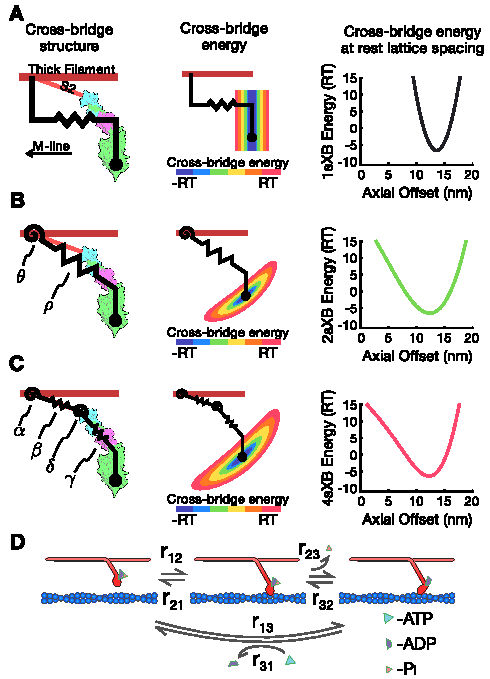
\includegraphics[width=3.1in]{../imgs/fig_xb_types.pdf}
    \caption{ \textbf{Cross-bridge types and kinetic scheme.} 
        (A)--(C) The three cross-bridge models, plotted against a myosin crystal structure for comparison (structure image generated from Gourinath et al.~(2003) \protect\citep{Gourinath2003} with PyMol \protect\citep{pymol}).
        The energy landscape of each cross-bridge and the free energy at rest lattice spacing are shown adjacent to the cross-bridge schematic.
        (A) The 1sXB introduced in Huxley (1957) \protect\citep{Huxley1957}. 
        (B) The 2sXB which uses a torsional/angular spring ($\theta$) and a linear spring ($\rho$). 
        (C) The 4sXB with two torsional and two linear springs.
        Of the 4sXB's springs, $\alpha$ corresponds to the point at which the S2 region rejoins the thick filament backbone, $\beta$ to the S2 region itself, $\delta$ to the area linking the S2 and the light chain domains, and $\gamma$ to the light chain domain itself.
        $\delta$ replicates the change in angle accompanying the power stroke by applying torque to the freely moving joint representing the converter domain.
        (D)  The three state kinetic system. 
        The three states represent (1) an unbound state, (2) a pre-power stroke state, and (3) a post-power stroke state. 
        The rate of transition between states $i$ and $j$ is represented as $r_{ij}$. 
        The forward and reverse transition rates are functions of energy stored in the cross-bridge. 
        \label{fig_xb_types}
        }
    \end{center}
\end{figure}

%\clearpage
\begin{figure}[!ht]
    \begin{center}
    %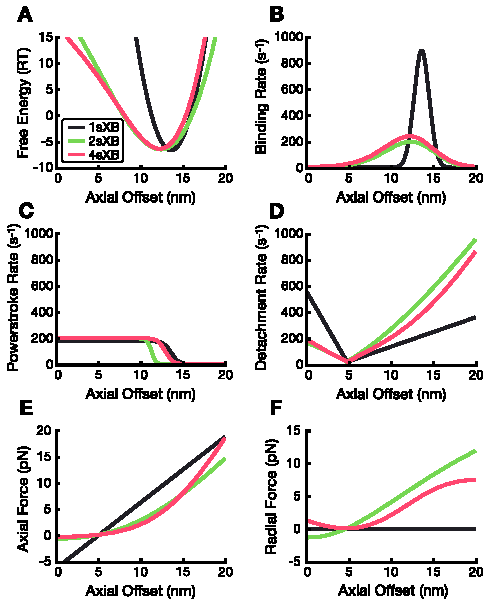
\includegraphics[width=3.25in]{../imgs/fig_kinetics_cuts.pdf}
    \caption{ \textbf{Forces, energy, and kinetics of the 1sXB, 2sXB, and 4sXB models at resting lattice spacing.}
        (A)--(F) show the energy, transition rates, and forces of the 1sXB model (black), 2sXB model (green), and 4sXB model (red) at resting lattice spacing.  
        The 1sXB model values shown for comparison are derived from those of Daniel et al.~(1998) and Tanner et al.~(2007), \protect\citep{Daniel1998, Tanner2007}, shifted axially so the resting location of the cross-bridge head in each case is aligned with the resting locations of the 2sXB model and 4sXB model allowing easier comparison. 
        The free energy of the cross-bridges in state two is shown in (A), where the multi-spring cross-bridges' shifts from a purely parabolic trajectory is visible. 
        The explicit two-dimensional thermal forcing of the multi-spring cross-bridge heads in (B) results in binding probabilities that are more distributed than those of the single spring cross-bridge.
        The rate of power strokes (C) remains least changed between the single and the multi-spring cross-bridge models.  
        The energy-based kinetics of the multi-spring cross-bridges are unable to fully replicate the biased detachment rate of the 1sXB model in (D).
        (E) and (F) show the 1sXB's sharp discontinuities in axial force and lack of any radial force.
        \label{fig_kinetics_cuts}
        }
    \end{center}
\end{figure}

%\clearpage
\begin{figure}[!ht]
    \begin{center}
    %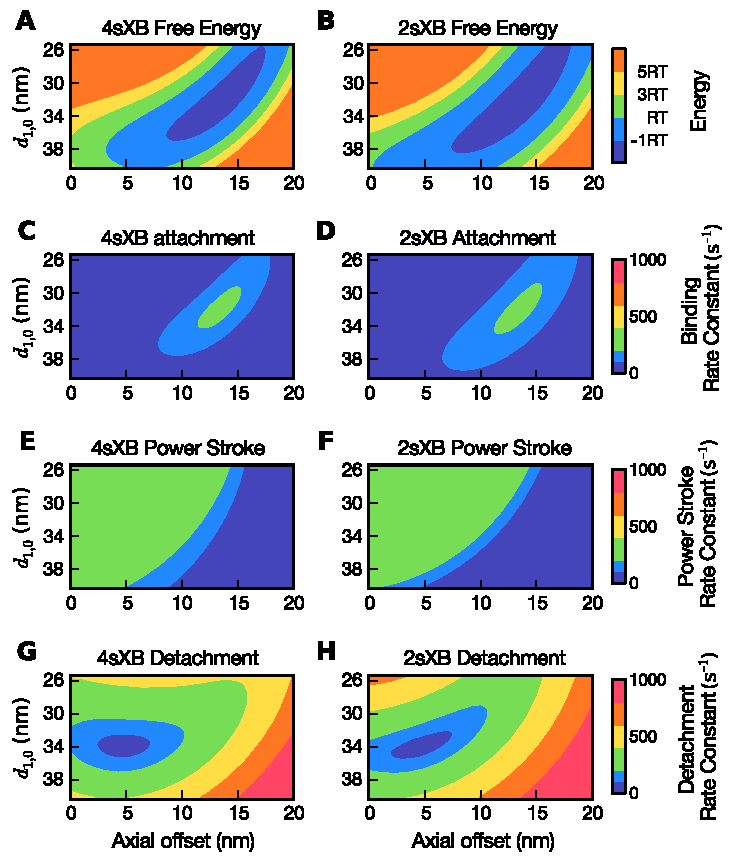
\includegraphics[width=3.25in]{../imgs/fig_kinetics_contours.pdf}
    \caption{ \textbf{Energy and kinetics of the multi-spring cross-bridge models change with axial offset and lattice spacing.} 
        Axial offset is the distance between the current axial location of the cross-bridge tip and the location where the cross-bridge attaches to the thick filament.  
        Lattice spacing ($d_{10}$) is defined as in Millman (1998) \protect\citep{Millman1998}, with an offset to account for filament thicknesses so the cross-bridge spans the filaments at a rest lattice spacing of 34 nm. 
        (A)--(H)  The properties of the 4sXB model (A, C, E, and G) and the 2sXB model (B, D, F, and H) as they change with binding site offset and lattice spacing.
        (A) depicts the free energy of the 4sXB model at various lattice spacings, with the head stretched to an axial offset from the thick filament attachment point.
        The free energy of the 2sXB model is shown in (B).  
        (C) and (D) show $r_{12}$, the probability that the 4sXB and 2sXB models will transition from an unbound state to a bound state. 
        (E) and (F) show $r_{23}$, the probability of transition from a pre-power stroke state to a post-power stroke state, for the same cross-bridges, axes, and scales as (C) and (D) show $r_{12}$.
        (G) and (H) show $r_{31}$, the probability of unbinding from a post-power stroke state. 
        The reverse rates, $r_{21}$, $r_{32}$, and $r_{13}$ are back-calculated from the forward rates.
        \label{fig_kinetics_contours}
        }
    \end{center}
\end{figure}

%\clearpage
\begin{figure}[!ht]
    \begin{center}
    %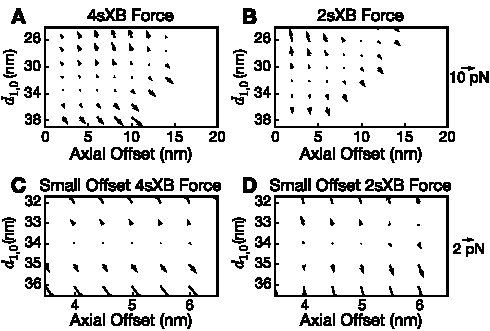
\includegraphics[width=3.25in]{../imgs/fig_forces.pdf}
    \caption{ \textbf{Overview and detail of the forces exerted by the 2sXB and 4sXB\@ models.}
        (A)--(D) show the forces exerted by the 4sXB and the 2sXB models; omitted are vectors for unlikely configurations as determined by the sum of $r_{23}$ and the inverse of $r_{31}$. 
        (A) and (B) show overviews of the forces exerted, respectively, by the 4sXB model and the 2sXB model over lattice spacings and axial offsets that vary as in Figure 2. 
        The forces exerted by the two cross-bridges have radial components which frequently equal or exceed their axial components. 
        A more detailed view of the region surrounding the rest position of the cross-bridges is shown in (C) and (D), where the large radial components of the cross-bridge forces, particularly for the 2sXB model, is again evident.  
        \label{fig_forces}
        }
    \end{center}
\end{figure}

%\clearpage
\begin{figure}[!ht]
    \begin{center}
    %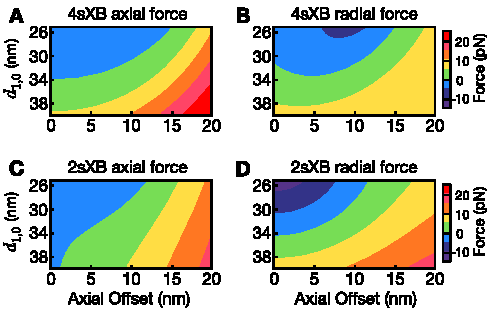
\includegraphics[width=8.3cm]{../imgs/fig_force_contours.pdf}
    \caption{ \textbf{Axial and radial forces as separate components.}
        (A)--(D) show, separated, the axial and radial components of the forces produced by the 4sXB and the 2sXB models.
        \label{fig_force_contours}
           }
    \end{center}
\end{figure}

%\clearpage
\begin{figure}[!ht]
    \begin{center}
    %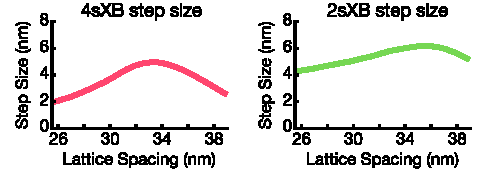
\includegraphics[width=8.3cm]{../imgs/fig_step_size.pdf}
    \caption{ \textbf{Changes in step size with lattice spacing.}
        Step size varies as lattice spacing diverges from its rest value.
        Step size is defined as the change in the rest axial offset between the pre- and post-power stroke states. 
        The 4sXB model and 2sXB model exhibit different tuning curves.
        \label{fig_step_size}
           }
    \end{center}
\end{figure}

%\clearpage
\begin{figure}[!ht]
    \begin{center}
    %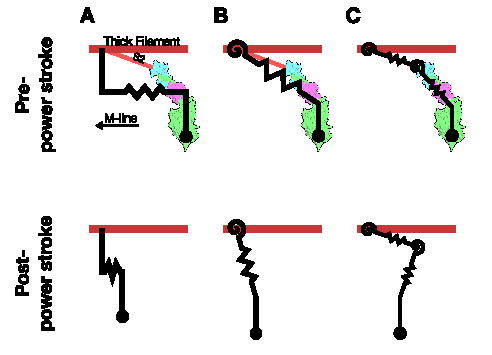
\includegraphics[width=8.3cm]{../imgs/fig_power_stroke_changes.pdf}
    \caption{ \textbf{Changes in cross-bridge resting geometry with the power stroke.}
        (A)--(C) show, schematically, the change in the rest lengths and angles of the single and multi-spring cross-bridges. 
        The rest length and angle of the 2sXB's extensional and torsional springs are set, in both the pre- and post-power stroke states so as to match the tip position of the 2sXB in each condition to that of the 4sXB (in Table~\ref{parameter_table}).
        The change in the unstressed radial distance from the thick filament to the tip of the multi-spring cross-bridges that occurs with the power stroke is particularly visible in (C) and (D) when compared to the single spring cross-bridge (A).
        The effects of the universal joint attaching the springs of the 4sXB and the 2sXB to the globular domain, and the globular domain's own fixed angle to the thin filament, are shown by the continued radial orientation of the globular domain after the power stroke occurs.
        \label{fig_power_stroke_changes}
           }
    \end{center}
\end{figure}

% section figure_legends (end)

\clearpage
\section*{Tables} % (fold)

\begin{table}[ht]
    \begin{center}
    \begin{tabular}[t]{|c|c|c|c|c|} \hline
    %\multicolumn{4}{|l|}{\textbf{4sXB}} \\ 
    %\multicolumn{1}{|l}{~} 
    Model & Spring    & Rest value & $E$        & Source \\ \hline % \cline{2-4}  
    4sXB  & $\alpha$  & 40\de      & 100 pN/rad & \citet{Liu2006}      \\ \hline
          & $\beta$   & 10.5 nm    & 10 pN/nm   & \citet{Liu2006}      \\ \hline
          & $\delta$  & 125\de     & 40 pN/rad  & \citet{Taylor1999}   \\ \hline
          & $\delta'$ & 70\de      & 40 pN/rad  & \citet{Taylor1999}   \\ \hline
          & $\gamma$  & 9.6 nm     & 5 pN/nm    & \citet{Houdusse2000} \\ \hline
    %\multicolumn{4}{|l|}{\textbf{2sXB}} \\ 
    %\multicolumn{1}{|l}{~} 
    %          & Rest value & $E$        & Source      \\ \cline{2-4} 
    2sXB  & $\theta$  & 47\de      & 40 pN/rad  & See caption \\ \hline
          & $\theta'$ & 73\de      & 40 pN/rad  & See caption \\ \hline
          & $\rho$    & 20 nm      & 2 pN/nm    & See caption \\ \hline
          & $\rho'$   & 16 nm      & 2 pN/nm    & See caption \\ \hline
    \end{tabular}
    \caption{ 
	    \label{parameter_table}
	    \textbf{Model parameters and their sources} 
	    Prime values, such as $\delta'$, represent post-power stroke state values. 
	    From Liu et al.~(2006) \citep{Liu2006}, which used insect flight muscle, the most frequently occurring thick filament to S2 angle range is 51-60\de. 
	    We assume that this range is being distorted by the compressive radial force being generated by the rigor cross-bridges in the swollen lattice spacings that Liu et al.~used. 
	    As such, we choose a rest angle for $\alpha$ at the low end of the still common range of 50\de~to 40\de. 
	    We do not change this angle between states one, two and three.
	    In Taylor et al.~(1999) \citep{Taylor1999} (clearly explained in \citep{Davis2009}) the angle between the LCD and the thick filament's axial axis goes from 125\de~to 70\de~with the power stroke. 
	    The LCD rest length generated by measurements made of structure 1DFK from Houdusse et al.~(2000) \citep{Houdusse2000}. 
	    The rest values of the 2sXB model's springs are determined by those of the 4sXB model; they are calculated so that the rest position of the 2sXB's head is the same as the rest position of the 4sXB's head. 
	    The spring constant, $E$, for the angular spring responsible for each cross-bridge's power stroke is determined by the change in angle over the power stroke and the energy liberated by the hydrolysis of ATP \citep{Tanner2007}. 
	    Additional spring constants are chosen to be consistent with previous work, and to provide sufficient flexibility to enable diffusion. 
    }
    \end{center}
\end{table}

% section tables (end)

\end{document}
